\documentclass[11pt]{memoir}

\usepackage{importationsprojet}

\pagestyle{empty}
\setlength{\parindent}{0pt}

\begin{document}

\begin{questions}

\exercice[18]
\par La production annuelle de déchets par Français était de \num{5,2} tonnes par habitant en 2007.\\
La production annuelle de déchets par Français était de \qty{4862}{kg} par habitant en 2007.\\
    \question De combien de \unit{kg} la production annuelle de déchets par Français en 2017 a-t-elle diminué par rapport à l'année 2007 ?
    \question Pour continuer à diminuer leur production de déchets, de nombreuses familles utilisent désormais un compositeur. Une de ces familles a choisi le modèle ci-contre, composé d'un pavé droit et d'un prisme droit (la figure du composteur n'est pas à l'échelle). Le descriptif indique qu'il a une contenance d'environ \qty{0.5}{\metre\cubed}. On souhaite vérifier cette information.
    \subpart Dans le trapèze $ABCD$, calculer la longueur $CH$.
    \subpart Montrer que la longueur $DH$ est égale à \qty{45}{\cm}.
    \subpart Vérifier que l'aire du trapèze $ABCD$ est de \qty{2385}{\cm\squared}.
    \subpart Calculer le volume du composteur. L'affirmation << il a une contenance d'environ \qty{0.5}{\m\cubed} >> est-elle vraie ?
    
    \begin{center}
        \begin{tikzpicture}
            \node[anchor=south west] at (0,2.7) {\textbf{Rappels :}};
            \draw (0,0) rectangle (16,2.7);
            \node[anchor=west] at (0,2) {Aire du trapèze $= \dfrac{(\textrm{Petit côté}+ \textrm{Grand côté}) \times \textrm{hauteur}}{2}$};
            \node[anchor=west] at (0,1) {Volume du prisme droit $=$ Aire de la base $\times$ hauteur};
            \node[anchor=west] at (0,0.3) {Volume du pavé droit $=$ Longueur $\times$ largeur $\times$ hauteur};
        \end{tikzpicture}
    \end{center}

\begin{center}
\begin{tikzpicture}[scale=1]
    \draw (0,0) -- (0,4) -- (3,4) -- (3,0) -- cycle;
    \draw (3,0) -- (4.5,1) -- (4.5,5) -- (3,4) -- cycle;
    
\end{tikzpicture}
\end{center}

\exercice[12]
\par Les points $B$, $D$ et $A$ sont alignés.\\
Les points $B$, $E$ et $C$ sont alignés.\\
La longueur $AC$ est égale à \qty{15}{\cm}.\\
$BA = \qty{12}{cm}$ ; $BC = \qty{9}{cm}$ ; $BD = \qty{8}{cm}$ ; $BE = \qty{6}{cm}$.\\
La figure ci-contre n'est pas à l'échelle.\\

\noindent Les affirmations suivantes sont-elles vraies ?\\
Justifier les réponses.

\vspace{1em}

\textbf{Affirmation 1 : } le triangle $ABC$ est rectangle en $B$.\\
\textbf{Affirmation 2 : } les droites $(AC)$ et $(DE)$ sont parallèles.

\begin{center}
    \begin{tikzpicture}[scale=0.5]
        \point{A}{(0,0)}
        \point{B}{(12,0)}
        \point{C}{(12,9)}[west]
        \point{D}{(4,0)}
        \point{E}{(12,6)}[west]
        \draw (A) -- (B) -- (C) -- cycle;
        \draw (D) -- (B) -- (E) -- cycle;
    \end{tikzpicture}
\end{center}

\exercice[9]
Les affirmations sont-elles vraies ? Justifier les réponses.
On considère la fonction $f$ définie par $f(x) = 2x+5$.

\textbf{Affirmation 3 :} L'antécédent de 6 par la fonction $f$ est égal à $\frac{1}{2}$.

On considère la fonction $f$ définie par $f(x) = 3x-7$
\textbf{Affirmation 4 :} L'image par $f$ du nombre $-1$ est $2$.

Un réacteur nucléaire a une puissance de \qty{900}{MW}.
Une centrale hydroélectrique a une puissance de \qty{9000}{kW}.
\textbf{Affirmation 5 :} il faut 10 centrales hydroélectriques pour obtenir la puissance d'un réacteur nucléaire.

\exercice[10]
\question Décomposer, sans justifier, en produit de facteurs premiers les nombres \num{1386} et \num{1716}.
\question En déduire la forme irréductible de la fraction $\dfrac{1386}{1716}$.

\exercice[25]
On veut peindre des murs d'aire inférieure à \qty{100}{m\squared}.
Voici les tarifs proposés par trois peintres en fonction de l'aire des murs à peindre en \unit{m\squared} :
\begin{itemize}
    \item Peintre A : \qty{150}{€} par \unit{\meter\squared}.
    \item Peintre B : \qty{100}{€} par \unit{\meter\squared} et \qty{1000}{€} d'installation de chantier.
    \item Peintre C : \qty{7000}{€} quelque soit l'aire inférieure à \qty{100}{\meter\squared}.
\end{itemize}

\question Montrer que pour \qty{30}{\meter\squared}, le tarif du peintre A est de \qty{4500}{€}, le tarif du peintre B est de \qty{4000}{€} et le tarif du peintre C est de \qty{7000}{€}.

Dans la suite de l'exercice, $x$ désigne l'aire des mur à peindre en \unit{\meter\squared}.

\question Écrire, en fonction de $x$, le prix proposé par le peintre B.

Les fonctions donnant les prix proposés par le peintre B et le peintre C sont représentés sur l'annexe 1.

\question Soient $A(x)$ et $B(x)$ les expressions des fonctions donnant le prix proposé par les peintres A et C en fonction de $x$. On a $A(x) = 150x$ et $C(x) = 7000$.
    \subpart Calculer l'image de $x$ par la fonction $A$.
    \subpart Calculer l'antécédent de $9000$ par la fonction $A$.
    \subpart Tracer la représentation graphique de la fonction $A$ sur l'annexe 1.
    
\question On a saisi dans un tableur les fonctions $A$, $B$ et $C$. Quelle formule a-t-on saisie en B2 puis étirée vers la droite ?

\question 
    \subpart Résoudre l'équation $150x = 100x+1000$.
    \subpart Interpréter le résultat de la question précédente.
    
\question Lire graphiquement, sur l'annexe, les surfaces entre lesquelles le peintre B est le moins cher des trois peintres.

\exercice[14]
\textit{Dans tout cet exercice, aucune justification n'est demandée.}
\textit{On rappelle que l'instruction \begin{scratch}\blockmove{s'orienter à \ovalnum{90}}\end{scratch} signifie que l'on s'oriente vers la droite.}

On donne le programme suivant :

\begin{scratch}
\blockinit{quand \greenflag est cliqué}
\blockpen{effacer tout}
\blockmove{aller à x:\ovalnum{0} y:\ovalnum{0}}
\blockmove{s'orienter à \ovalnum{90}}
\blockrepeat{répéter \ovalnum{4} fois}
{
    \blockmoreblocks{Triangle}
    \blockmove{avancer de \ovalnum{50}}
}
\end{scratch}
\begin{scratch}
\initmoreblocks{définir \namemoreblocks{Triangle}}
\blockpen{stylo en position d'écriture}
\blockrepeat{répéter \ovalnum{3} fois}
{
    \blockmove{avancer de \ovalnum{50}}
    \blockmove{tourner \turnright{} de \ovalnum{90} degrés}
}
\end{scratch}

\end{questions}


\end{document}